%%%%%%%%%%%%%%%%%%%%%%%%%%%%%%%%%%%%%%%%%%%%%%%%%%%%%%%%%%%%%%%%%%%
% Method
% Team:
% Union
% Members: 
% Bernie Huang, Jim Lan, Hoang Tan, Kenny Hsu, Rahul Aditya, Tan Phat, Wei
% Relative files:
% Method_Union.tex
% Note:    
% Do not compile this file compile Main.tex to get the pdf file instead.
%%%%%%%%%%%%%%%%%%%%%%%%%%%%%%%%%%%%%%%%%%%%%%%%%%%%%%%%%%%%%%%%%%%
	
\subsection*{Title extraction}
Using python to catch the title. First step, we import some necessary packages and function.
\begin{enumerate}
	\item re: Regular expression package
	\item os: this function could connect the python to operating system so that we can call the path
	\item nltk: natural language toolkit, we use the corpus plaintext function to build the txt file in a folder as corpus
\end{enumerate}  
Second step,we convert every PDF file we want to deal with into txt file and set the path and store them in specific folder.
Third step,ues regular expression in python to capture the first sentence in the txt files which have been convertrd and stored in specific folder in previous step. 
Fourth step, output the title of the article in txt file.   

\subsubsection*{Author extraction}


\subsubsection*{Abstract extraction}
	I use the python to catch the abstract.
	\begin{center}
		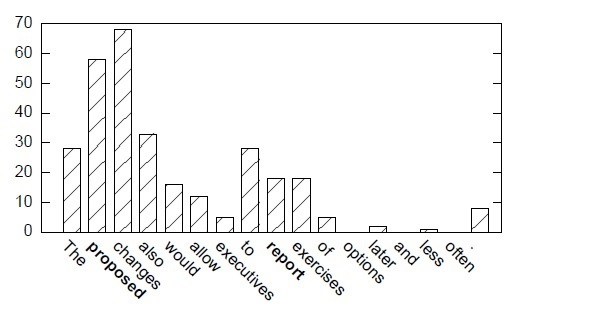
\includegraphics[width=0.8\columnwidth]{Union_Background_Chart_2}
	\end{center}
	The pdf is converted into txt file.Thus, it will create the txt file. The work is done by hand coding. For detailed coding scheme, we have presented it in the appendix at the end of this report\\ 
	After being able to read the txt file on every line, the python detects the abstract-database's words ,it will start to catch the sentences.\\ 	
	abstract-database:including the condition\\
	1. capital         "ABSTRACT"\\
	2. lower case      "abstract"\\
	3. in the sentence "Abstract—Word sense ....."\\
	4. and so on \\
	In the process building "abstract database", we are aware of different papers may have different form of structures and writing style, we search through numbers of articles from different journals. Number of article found is 100, from 20 different journals including The Lancet, Progress in Energy and Combustion Science, Chemical Analysis and so. Search results for sections such as Theoretical, Methods, Results, Discussion, Conclusion, Acknowledgements are also obtained.  Table below are the results of the search.\\
	\begin{table}
		\includegraphics{Table for method Union}.\\
		\includegraphics{Table 2 for method Union}.\\
		\caption{Result of finding all forms of "abstract", "introduction" written by different authors}
	\end{table}
	Then the our program will read the txt file on every line.If the python detects the abstract-database-stop's words ,it will stop to catch the sentences.\\ 
	abstract-database-stop:including the following conditions
	1. the blank line
	2. specific words in the beginning "Keywords"
	3. and so on.\\
	The intended output are sentences extracted to the txt file. To further validate if the program can run precisely, members randomly search for articles (10 articles) to test the programs. The program was run successfully and all abstracts was extracted from the text. \\ 	
	
\end{itemize}

\subsubsection*{Search sentences}
\begin{itemize}
	\item I use python to complete the task. 
	\begin{center}
		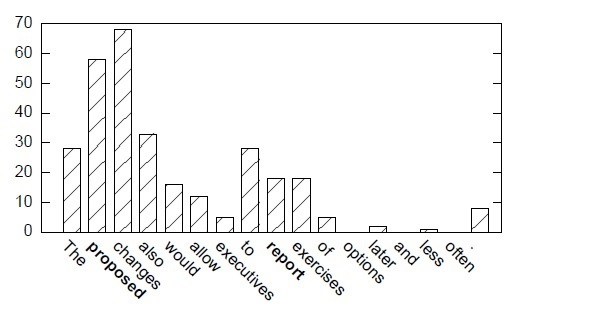
\includegraphics[width=0.8\columnwidth]{Union_Background_Chart_2}
	\end{center}
	\item First,turn the PDF to the txt file .(Make the programe easy to read file)\\ 
	\item Second,read the txt file by lines.\\ 	
	\item Third,create the array to divide the section of the articles.\\ 	
	\item Forth,expend the array to divide the section clearly.\\ 	
	\item Fifth,Users search the sentence.The programe search all sections by this sentence.\\
	\item Sixth,Show the results\\  		
	
\end{itemize}

\newpage % Ends the current page and causes all figures and tables to be printed